% arara: pdflatex
% arara: pdflatex
% arara: pdflatex

% options:
% thesis=B bachelor's thesis
% thesis=M master's thesis
% czech thesis in Czech language
% slovak thesis in Slovak language
% english thesis in English language
% hidelinks remove colour boxes around hyperlinks

\documentclass[thesis=M,czech]{FITthesis}[2019/12/23]
\usepackage{minted}
\makeatletter\AtBeginDocument{\let\@elt\relax}\makeatother

\usepackage[utf8]{inputenc} % LaTeX source encoded as UTF-8

\usepackage{amsmath} %advanced maths
\usepackage{amssymb} %additional math symbols

\usepackage{graphicx}
\graphicspath{ {./img/} }

\usepackage{dirtree} %directory tree visualisation
\RequirePackage{pdfpages}

% % list of acronyms
% \usepackage[acronym,nonumberlist,toc,numberedsection=autolabel]{glossaries}
% \iflanguage{czech}{\renewcommand*{\acronymname}{Seznam pou{\v z}it{\' y}ch zkratek}}{}
% \makeglossaries

\newcommand{\tg}{\mathop{\mathrm{tg}}} %cesky tangens
\newcommand{\cotg}{\mathop{\mathrm{cotg}}} %cesky cotangens

% % % % % % % % % % % % % % % % % % % % % % % % % % % % % % 
% ODTUD DAL VSE ZMENTE
% % % % % % % % % % % % % % % % % % % % % % % % % % % % % % 

\department{Katedra softwarového inženýrství}
\title{Srovnání REST, GraphQL a gRPC API v~Node.js}
\authorGN{Tomáš} %(křestní) jméno (jména) autora
\authorFN{Buňata} %příjmení autora
\authorWithDegrees{Bc. Tomáš Buňata} %jméno autora včetně současných akademických titulů
\author{Tomáš Buňata} %jméno autora bez akademických titulů
\supervisor{Ing. Lukáš Loukota}
\acknowledgements{Doplňte, máte-li komu a za co děkovat. V~opačném případě úplně odstraňte tento příkaz.}
\abstractCS{V~několika větách shrňte obsah a přínos této práce v~češtině. Po přečtení abstraktu by se čtenář měl mít čtenář dost informací pro rozhodnutí, zda chce Vaši práci číst.}
\abstractEN{Sem doplňte ekvivalent abstraktu Vaší práce v~angličtině.}
\placeForDeclarationOfAuthenticity{V~Praze}
\declarationOfAuthenticityOption{4} %volba Prohlášení (číslo 1-6)
\keywordsCS{Nahraďte seznamem klíčových slov v češtině oddělených čárkou.}
\keywordsEN{Nahraďte seznamem klíčových slov v angličtině oddělených čárkou.}
% \website{http://site.example/thesis} %volitelná URL práce, objeví se v tiráži - úplně odstraňte, nemáte-li URL práce

\begin{document}

% \newacronym{CVUT}{{\v C}VUT}{{\v C}esk{\' e} vysok{\' e} u{\v c}en{\' i} technick{\' e} v Praze}
% \newacronym{FIT}{FIT}{Fakulta informa{\v c}n{\' i}ch technologi{\' i}}

\begin{introduction}
Webové aplikace jsou každodenní součástí našeho života. Setkáváme se s nimi při čtení ranních zpráv, komunikaci se svými přáteli nebo spravování financí přes internetové bankovnictví.
Architektura webových aplikací se dá rozdělit na dvě hlavní části: frontend (část se kterou interaguje uživatel v prohlížeči) a backend (serverová část, která slouží k ukládání a  manipulaci s daty). V této práci se věnuji té druhé části - konkrétně backendovým technologiím zprostředkovávající komunikaci mezi serverem a klientem.
Vzhledem k tomu, že webové technologie se velmi rychle vyvíjejí a posouvají vpřed, vývojáři velmi často narážejí na otázku výběru správné technologie pro svůj projekt. V této práci se pokusím na tuto otázku odpovědět. Porovnám mezi sebou následující: REST, GraphQL a gRPC.

REST je z těchto technologií nejstarší a v současnosti také nejpopulárnější. Princip RESTu je takový, že každá entita je identifikována unikátním URI a pomocí HTTP metod je s těmito entitami manipulováno.
GraphQL vzniklo přibližně o deset let později a funguje zcela na odlišném principu - vystavuje jediný endpoint, na který se poté dotazujeme speciálním jazykem, který strukturou velmi přípomína JSON.
gRPC je z těchto technologií nejmladší a jedná se o open source implementaci RPC (volání vzdálené procedury) od společnosti Google.

S každou z těchto technologií implementuji aplikační rozhraní pro eshop a následně je porovnám ze stránek uživatelské zkušenosti, podpory vývojářů a míry schopnosti zvládat zátěž.
V teoretické části práce se budu věnovat představení těchto technologií. Poté se budu věnovat požadavkům na návrh backendu aplikace, na kterém tyto technologie budou demonstrovány. Další část se bude věnovat výběru databázového systému a dalších technologií potřebných pro správné fungování aplikace.
V praktické části se budu nejdříve věnovat implementaci jednotlivých backendů, včetně otestování jejich správné funkčnosti, a poté otestuji jejich výkon zátěžovými testy. Poslední část se bude věnovat věnovat samotnému srovnání těchto technologií.

\end{introduction}

\chapter{Cíl práce}
Cílem práce je návrh a implementace  tří shodných API v REST, GraphQL a gRPC, která budou realizovat typické operace, které využívají eshopy - např. vytvoření účtu zákazníka, listování produktů nebo vytvoření objednávky. Tato API budou implementována nad Node.js.

Teoretická část se zabývá samotným návrhem API, kde jsou prozkoumány různé služby, které by měly být integrované do systému. Návrh vychází z typických operací potřebných pro chod eshopu. V této části budou také popsány použité technologie.

Cílem praktické části je implementace je navázat na předchozí část implementací navrženého API. Bude ukázány klíčové implementační kroky, které jsou potřeba pro realizaci API v daných technologií. Součástí implementace je také napsání testů, které ověří funkčnost vytvořených systémů.\\
Dále zde bude popsána metodologie porovnání (dokumentace, rychlost vývoje, výkonnostní testování, ...) a na základě této metodologie budou tyto technologie porovnány.



\chapter{Analýza}
Před tím, než se začneme věnovat návrhu a implementaci API, je v hodné si nejdříve vysvětlit co znamená pojem API a následně představím co to je REST, GraphQL a gRPC. Současně také popíšu jaké knihovny jsem si vybral pro jejich implementaci. A poté představím samotný návrh API, které bude implementováno v praktické části.

\section{API}
Zkratka API označuje rozhraní pro programování aplikací. Jedná se o velmi důležitou součást vývoje, protože definuje způsob jak mezi sebou budou jednotlivé aplikace (nebo komponenty v rámci jedné aplikace) komunikovat. Dalo by se říci, že představuje smlouvu, kterou obě strany musí dodržet abz spolu mohli komunikovat\\
API se skládá ze dvou částí: 
\begin{itemize}
    \item Technické specifikace, která popisuje možnosti komunikace - metody, které API vystavuje, vstupní data...
    \item Softwarového rozhraní, které tuto specifikaci implementuje
\end{itemize}

API se dále mohou dělit podle dostupnosti na soukromá, partnerská nebo otevřená. Soukromá API se používají výhradně v rámci jedné organizace. Ikdyž aplikace, které tato API využívají mohou být veřejně dostupné, samotné rozhraní není.\\
Partnerská APi jsou sdílená s business partnery a slouží hlavně k integraci systémů mezi partnery a společností, která poskytuje přístup k API.\\
Otevřená API jsou volně dostupná všem vývojářům a je možné je využívat bez explicitního souhlasu poskytovatele těchto rozhraní nebo bez licenčních poplatků. Poplatky mohou být účtované za informace dostupné za rozhraním, ale dokumentace  a testovací data musí být veřejně dostupná.

Aplikační programovací rozhraní jdou také dělit podle způsobu použití. Může se jednat třeba o databázové API, které umožnuje komunikaci mezi aplikací a databázovým systémem, nebo API operačního systému, které definuje jak programy mohou využívat zdroje a služby operačního systému.\\
Nejběžnější, a z pohledu této práce také nejzajímavější, jsou však webová aplikační rozhraní, která poskytují data a funkcionality mezi webovými systémy reprezentující architekturu klient-server. Tato API typicky doručují požadavky z webových aplikací a odpovědi ze serverů prostřednictvím protokolu HTTP. Mezi jeden z nejpopulárnějších typů webových aplikační rozhraní patří REST, ikdyž v poslední době jeho popularita začíná pomalu klesat, viz obrázek \ref{google_trends_img} \cite{google-trends}.

\begin{figure}[h]
    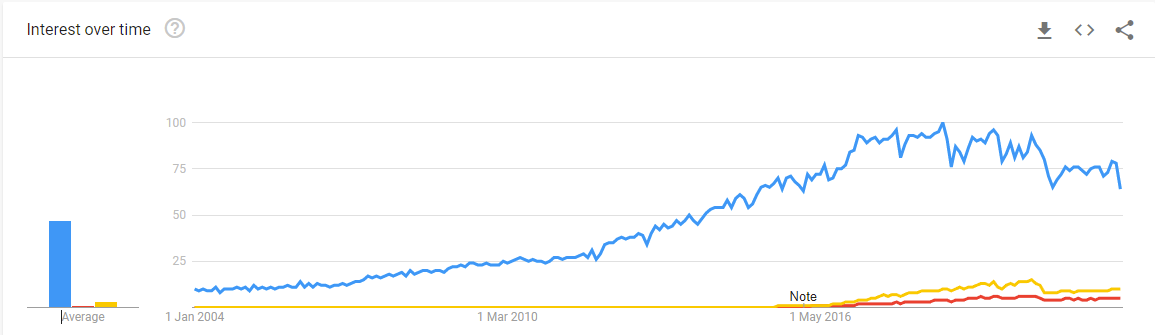
\includegraphics[width=\linewidth]{img/interest_trend.png}
    \caption{Google Trends: REST (modrá), GraphQL (žlutá) a gRPC (červená)}
	\label{google_trends_img}
\end{figure}

\section{REST}
REST je velmi oblíbený architektonický styl pro tvorbu API, který vyniká svou jednoduchostí a čitelností. Na rozdíl např. od gRPC není orientován procedurálně, ale datově.\\
Zkratka REST vyjadřuje pojem representational state transfer a v roce 2000 ji zavedl Roy Fielding ve své dizertační práci \cite{fielding00}. Než si vysvětlíme, jaké požadavkz musí REST API splňovat, je potřeba vysvětlit co to je zdroj.\\
Jakákoli informace, kterou lze pojmenovat, může být zdrojem. Může to být například obrázek, dočasná služba nebo kolekce jiných zdrojů. Stav zdroje v čase nazýváme reprezentace zdroje. Skládá se ze tří částí - dat, metadat popisující tato data a hypermedia odkazů, která pomáhají klientům s přechodem do dalšho požadovaného stavu.

Aby aplikační rozhraní mohlo být nazýváno RESTful, je potřeba aby splňovalo šest architektonických omezení \cite{restful_api}:

\subsection{Uniform Interface}
Aplikováním principu generality na rozhraní komponenty můžeme zjednodušit architekturu celého systému. Tomu pomáhá několik omezení.
\begin{itemize}
    \item \textbf{Identifikace zdrojů} - Rozhraní musí jednoznačně identifikovat každý zdroj, který je použit v interakci mezi klientem a serverem
    \item \textbf{Manipulace se zdroji} skrz jejich reprezentaci - Zdroje v odpovědi serveru by měly mít jednotnou reprezentaci. Konzumenti API by pak měli použít tyto reprezentace k modifikování stavu zdrojů.
    \item \textbf{Samopopisující se zprávy} - Každá reprezentace zdroje by měla obsahovat dostatek informací aby bylo jasné jak ji zpracovat. Měla by také obsahovat jaké další možné operace může klient se zdrojem provádět.
    \item \textbf{Hypermedia jako aplikační stav} - Klient by měl mít pouze počáteční URI aplikace. Klientská aplikace by poté měla řídit veškeré interakce pomocí hyperlinků - serverová odpověď obsahuje seznam dostupných operací.
\end{itemize}

\subsection{Client-server}
Návrhový vzor klient-server vynucuje oddělení zodpovědností, což pomáhá tomu aby se klientské a serverové komponenty mohly vyvíjet nezávisle na sobě. Zatímco se server a klient vyvíjí, je potřeba dávat pozor, aby rozhraní mezi nimi nebylo porušeno.
Oddělením uživatelského rozhraní (klienta) a manipulaci s daty (serveru) umožníme nezávislost uživatelského rozhraní na konkrétní platformě a zároveň zlepšíme škálovatelnost serveru zjednodušením jeho komponent. Servery nebo klienti mohou být také nahrazeny, pokud nedojde ke změně rozhraní

\subsection{Stateless}
Bezestavovost požaduje, že každý požadavek z klienta na server musí obsahovat všechny dostupné informace potřebné k jeho zpracování. Server nemůže využívat žádných uložených informací z předchozích interakcí - chová se jako kdybz každý požadavek byl úplně nový. Z toho vyplývá, že klient je zodpovědný za udržování aplikačního stavu, pokud to je potřeba.

\subsection{Cacheable}
Toto omezení požaduje, že každá odpověď serveru by se měla označit jako cachovatelná nebo necachovatelná. Pokud je cachovatelná, klient má po omezenou dobu právo tyto informace přepoužít v dalších požadavcích

\subsection{Layered system}
REST umožnuje využití vrstvené architektury, kde například server A obsahuje API, na serveru B se ukládají data a na serveru C se autentizují požadavky. Klient nemůže zjistit, jestli je ke konkrétnímu serveru připojen přímo nebo přes prostřeníka.

\subsection{Code on demand - volitelné}
Umožnění rozšíření funkcionality klienta stažením a spuštěním kódu ve formě appletů nebo skriptů ze serveru. Výsledkem je zjednodušení klienta, který nemusí obsahovat tolik předinstalovaných funkcí.

\subsection{HTTP}
Pro přenos dat mezi klientem a servrem se nejčastěji používá protokol HTTP, ikdyž REST není vázaný na tento protokol. Protože ale se tato práce zabývá pouze webovými API, budu se v této práci věnovat pouze přenosu pomocí HTTP.
HTTP definuje množinu metod, které slouží k indikaci jakou akci chceme se zdrojem provést. Tyto metody se také označují jako \textit{HTTP verbs} \cite{http_metods}

\begin{itemize}
    \item \textbf{GET} - slouží k získání reprezentace daného zdroje. Měla by být použita pouze k získávání informací.
    \item \textbf{HEAD} - slouží k získání stejné odpovědi jako \textbf{GET}, ale bez těla odpovědi.
    \item \textbf{POST} - slouží k odeslání entity k danému zdroji, která často způsobí změnu stavu nebo side-effect na serveru.
    \item \textbf{PUT} - tato meto nahradí všechny současné reprezentace cílového zdroje za obsah požadavku
    \item \textbf{DELETE} - slouží ke smazání cílového zdroje.
    \item \textbf{PATCH} - slouží k částečné změně cílového zdroje
\end{itemize}

Metody, které nemění stav serveru označujeme jako bezpečné. Jedná se hlavně o GET a HEAD. V praxi ale bežně není možné tyto metody na straně serveru implementovat tak, aby neměnily vůbec žádný stav - může například dojít k zalogování metody nebo obnovení cache.

Další kategorie jsou idempotetní metody. Idempotence znamená, že pokud klient provede několik shodných požadavků, všechny budou mít stejný výsledek. Jedná se hlavne o GET, HEAD, PUT a DELETE. To ale neznamená, že server musí na každý požadavek odpovědět stejně.


\subsubsection*{Stavové kódy}
HTTP taktéž definuje stavové kódy odpovědí. Tyto kódy se v REST api využívají k informování klienta o výsledku prováděné operace. Tyto kódy se dělí do pěti kategorií, které se od sebe liší prvním číslem. Kódy s začínající číslem 100 jsou informační - komunikují informace na úrovni transportního protokolu \cite{http_codes}. Kódy začínající číslem 200 informují o úspěšném zpracování požadavku. Kódy s číslem 300 značí, že je potřeba dodatečná akce od klienta. Číslo 400 označuje chybový stav na straně klienta. Poslední jsou pak kódy s číslem 500, které označují chybu na straně serveru. Nejčastěji se setkáme s následujícími kódy:
\begin{itemize}
    \item 200 OK - Požadavek proběhl v pořádku. Na rozdíl od kódu 204 by odpověď měla obsahovat i data, a je závislá na použité metodě. Například pro GET by se mělo jednat o reprezentaci zdroje, zatímco pro POST se může jednat o výsledek operace. %todo%
    \item 201 Created - Požadavek proběhl v pořádku a jeho výsledkem je vytvoření zdroje. Typicky se jedná o vytvoření zdroje uvnitř kolekce pomocí POST metody.
    \item 204 No Content - Server naplnil požadavek, ale není potřeba vrátit žádnou hodnotu. Například při operaci DELETE, kdy mažeme zdroj z kolekce. Tělo odpovědi nesmí obsahovat žádná data.
    \item 400 Bad Request - Požadavek je pro server nečitelný. Jedná se o obecný chybový kód, který se použije pokud žádný jiný není vhodný. Může se například jednat o špatný formát požadavku. Klient by stejný požadavek neměl opakovat beze změny.
    \item 401 Unauthorized - Klient není ověřen. Požadavek může být opakován s doplněnými informacemi o oveření.
    \item 403 Forbidden - Klient nemá dostatečná práva. Narozdíl od 401, identita klienta je známa.
    \item 404 Not Found - Server nenašel požadovaný zdroj.
    \item 405 Method Not Allowed - Klient použil metodu, kterou daný zdroj nepodporuje. Odpověď musí obsahovat hlavičku s výčtem podporovaných metod.
    \item 500 Internal Server Error - Server narazil na neočekávanou chybu při zpracování požadavku. Jedná se o obecný chybový kód. Nikdy se nejedná o chybu klienta a dává smysl stejný požadavek opakovat s očekáváním jiné odpovědi.
    \item 503 Service Unavailable - Server není připravený zpracovat požadavek.
\end{itemize}

\section{GraphQL}
GraphQL bylo vytvořeno společností Facebook v roce 2012. Hlavním důvodem jeho vzniku byla narůstající potřeba API pro získávání dat, které bude dostatečně silné a zároveň bude jednoduché na používání. V roce 2015 pak bylo GraphQL zpřístupněno jako opensource \cite{graphql_fb}. Od této doby vznikla spousta implementací v různých jazycích jako je Javascript, Java, Python a mnoha dalších. GraphQL sestává z typového systému, dotazovacího jazyka, statické validace a typové introspekce.

\subsection{Základní vlastnosti}
\subsubsection*{Definuje strukturu dat}
První věcí, kterou si na GraphQL můžeme všimout je to, že struktura dat posílaných na server se velmi podobá struktuře dat vrácených v odpovědi, viz obrázek \ref{graphql-query}. To přispívá ke zjednošení psaní dotazů - pokud víme jaká data server potřebuje - a také víme jaký formát dat očekávat. To je jedna z velkých výhod GraphQL, klient si určuje formát dat posílaných ze serveru a má tak přizpůsobená data pro své požadavky.

\begin{figure}[h]
    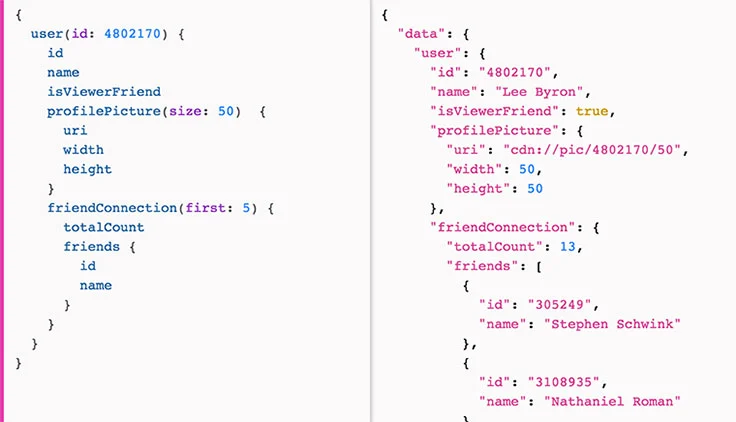
\includegraphics[width=\linewidth]{img/graphql-query.png}
    \caption{Příklad GraphQL dotazu a odpovědi \cite{graphql_query_img}}
	\label{graphql-query}
\end{figure}

\subsubsection*{Hierarchický}
Dalším důležitým apektem GraphQL je jeho hierarchičnost. Přirozeně totiž sleduje vztahy mezi objekty a oproti RESTu tak dovoluje vyhnout se několikanásobnému volání API pro získání dat souvisejících objektů.

\subsubsection*{Silně typový}
Každý GraphQL server definuje typový systém, který je specifický pro aplikaci.
Každá úroveň GraphQL dotazu odpovídá určitému typu a každý typ má definovanou množinu atributů, které obsahuje. Toto umožňuje validaci dotazů ještě před odesláním na server a zobrazování relevantních chybových hlášek.

\subsection*{Protokol, ne úložiště}
Každému atributu v GraphQL na serveru odpovídá nějaká funkce. Pokud už máme existující logiku aplikace společně s úložištěm, můžeme toto všechno na GraphQL napojit.

\subsection*{Introspekce}
Díky typovému systému máme možnost prozkoumávat schéma a zjistit dostupné \textit{queries}, \textit{mutace} nebo \textit{subscriptions}. Schéma také slouží jako smlouva mezi frontendem a backendem definující jak spolu budou komunikovat.
Introspekce také vytváří platformu pro různé nástroje - od generování kódu po tvorbu dokumentace.

\subsubsection*{Bez verzí}
Pokud v REST API chceeme zachovat stávající funkčnost klientů při přidávání nových funkcionalit, je potřeba zavést verzování API. V praxi je to často řešeno prefixem s číslem verze v URI zdroje, např. \mintinline{text}{http:localhost/v1/products}. S přibývajícím počtem verzí pak roste náročnost úprav API - pokud budeme například opravovat chybu v aplikaci, je potřeba zajistit, že chyba bude opravena ve všech verzích API, což je velmi časově náročné.

Pokud v GraphQL navrhneme API chytře, tomuto problému se vyhneme. Protože klient si určuje podobu dat sám, server může být jednodušší a obecnější. Místo upravování stávajících funkcionalit, které by poškodily stávající kompatibilitu, budeme přidávat nové. Tento přístup funguje hlavně proto, že podobu vrácených dat si určuje klient, což zabrání případnému nabobtnávání. Atributy, které dále už nebudou podporovány mohou být označeny dekorátorem \mintinline{text}{@deprecated} jako zastaralé a dále budou fungovat aby nebyla porušena zpětná kompatibilita. Díky těmto postupným změnám máme možnost vyhnout se verzování API.

\subsection{Typový systém}
Protože GraphQL není závislé na konkrétním programovacím jazyku, definuje svoje vlastní typové schéma - typicky v souboru \mintinline{text}{schema.gql}
Hlavním stavebním prvek schémat je \textit{Object type}. To je obecný typ, který obsahuje několik dalších atributů. Jeho definice může vypadat následovně. 
\begin{figure}[h]
\begin{minted}{gql.py:GraphqlLexer -x}
    type Cart {
        id: Float!
        items: [CartItem!]!
        totalPrice: Float!
        userId: Float!
    }
\end{minted}
\end{figure}
\begin{itemize}
    \item \textbf{Cart} definuje \textit{Object type}
    \item \textbf{id} je typu Float. Vykřičník znamená, že tento artibut je \textit{non-nullable}, což slibuje, že hodnota vždy bude odpovídat danému typu, v tomto případě \textit{Float}
    \item \textbf{items} reprezentuje pole typu \textit{CartItem}. CartItem je další uživatelem definovaný \textit{Object type}
    \item \textbf{totalPrice} a \textbf{userId} jsou opět typu \textit{Float}
\end{itemize}

Každý atribut typu \textit{Object type} může mít libovolný počet argumentů. Každý z těchto argumentů má své jméno. Narozdíl třeba od Javascriptu, kde funkce přebírají seznam seřazených argumentů, v GraphQL jsou předávány jménem.

Ikdyž ve schématu bude nejvíce zastoupen \textit{Object type}, existují ještě tři velmi důležité typy - \textit{Query}, \textit{Mutation} a \textit{Subscription}. Jedná se o jediné typy operací, které v GraphQL můžeme provádět.

Query se používá pouze pro čtení dat ze serveru, nesmí měnit stav serveru. Mutation se naopak používá právě když je potřeba stav serveru modifikovat. Přirovnáme-li to k RESTu, query jsou obdobou k metodě \mintinline{text}{GET} a mutation k \mintinline{text}{POST}, \mintinline{text}{PUT} nebo \mintinline{text}{DELETE}. Mutation také může vracet data, ale ta by měla být relevantní k provádené operaci.
Posledním typem je Subscription. Stějně jako dotazy, subscription slouží k získávání dat, ale rozdíl je v tom, že se jedná o dlouho trvající operace. Udržují aktivní spojení se serverem a umožňují tak serveru notifikovat klienta o změnách objektů, ke kterým se přihlásil. Subscription jsou vhodné hlavně pro real-time data - například sledování ceny akcií.

\begin{minted}{gql.py:GraphqlLexer -x}
type Query {    
    getProduct(id: Float!): Product!
}

type Mutation {
    addProduct(newProductData: NewProductInput!): Product!
}
\end{minted}

Na příkladě výše máme definováno jedno query \mintinline{text}{getProduct}, které slouží k získání detailu produktu podle jeho identifikátoru. Níže je pak definována mutation \mintinline{text}{addProduct}, která slouží k vytvoření nového produktu na základě uživatelského vstupu. Můžeme si všimnout, že tyto typy si jsou velmi podobné - největší rozdíl je v názvu operace.

Stavebním prvek typového systému je typ \textit{Scalar}, reprezentující listy listy dotazů. Mezi skalární typy v GraphQL patří:
\begin{itemize}
    \item Int: celé číslo
    \item Float: desetinné číslo se znaménkem
    \item String: UTF-8 zakódovaný řetězec
    \item Boolean: hodnota true nebo false
\end{itemize}
V mnoha implementacích GraphQL existuje možnost pro definici vlastních skalárních typů. Často je potřeba definovat si typ pro reprezentaci data a času. Je pak naší zodpovědností zajistit serializaci, deserializaci a validaci tohoto typu. Výčtový typ \textit{Enum} je speciálním skalárním typem a slouží reprezentaci dat, která mohou nabývat pouze několika předem daných hodnot. 

Typ \textit{Input} pak ještě slouží slouží k definování dat, která poskytuje uživatel v dotazu a má podobné vlastnosti jako \textit{Object type}
\begin{minted}{gql.py:GraphqlLexer -x}
    type Query {    
        getProduct(id: Float!): Product!
    }
    
    type Mutation {
        addProduct(newProductData: NewProductInput!): Product!
    }
\end{minted}

\subsection{Dotazovací jazyk}
GraphQL je deklarativní jazyk. To znamená, že specifikujeme jak výsledek má vypadat, místo postupu jak by měl být nalezen. Nejlépe si to ukážeme na příkladu. Uvažujme následující dotaz:

\begin{figure}[h]
\begin{minted}{gql.py:GraphqlLexer -x}
query {
    allProducts(productFilterData: { minPrice: 20, maxPrice: 100 }) {
        id
        name
        price
        status {
            id
            name
        }
    }
}
\end{minted}
\end{figure}

Na první řádce specifikujeme, že se jedná o dotaz. Dále je pak potřeba specifikovat jméno dotazu \mintinline{text}{allProducts}, za kterým následuje objekt se vstupními daty pro filtrování produktů - v tomto případě se jedná o minimální a maximální cenu produktu - \mintinline{text}{minPrice} a \mintinline{text}{maxPrice}. Poté už jen následuje objekt se samotným výčtem atributů, jejichž hodnoty chceme získat.

Můžeme si všimnout, že atribut \mintinline{text}{status} je typu objekt. Protože všechny typy listů dotazu musí být skalární objekty, je zde potřeba určit nějakou podmnožinu atributů, které skalární budou, jinak by dotaz skončil chybou. Aby se dotaz mohl vyhodnotit, je vždy potřeba specifikovat alespoň jeden atribut.

Na příkladu níže můžeme vidět výsledek tohoto dotazu. Pokud se podařilo dotaz v pořádku provést, najdeme odpověd vždy v objektu \mintinline{text}{data}. Snadno nahlédneme, že odpověď serveru je skutečně velmi podobná struktuře původního dotazu. Hlavními rozdíly jsou absence vstupních dat a to, že produkt je obalený v hranatých závorkách - to proto, že tento dotaz vrací pole objektů.

\begin{minted}{js}
{
  "data": {
    "allProducts": [
      {
        "id": 2,
        "name": "Striped Cotton-Blend Socks",
        "price": 25,
        "status": {
          "id": 1,
          "name": "New"
        }
      }
    ]
  }
}  
\end{minted}

\subsection{Statická validace}
Díky definovanému schématu je jednoduché validovat dotazy - klient snadno rozpozná zda nějaký dotaz je validní, a to právě ještě před odesláním na server. Typickými chybami mohou být chybějící vstupní data, přistupování k atributům nějakého skalárního atributu nebo naopak nepřistupování k žádnému atributu neskalárního objektu.

\subsection{Introspekce}
Introspekce nám dovoluje dotazovat API pro informace a schématu bez toho abychom museli číst dokumentaci. Můžeme si tak zobrazit dotazy, typy atributy nebo direktivy, které server podporuje. Velmi to usnadní práci vývojářům, ale pokud se k našemu API dostane nějaký útočník, dostává zdarma dokumentaci jak server využít. Je tedy vhodné introspekci zakázat v produkčním prostředí.
Introspekci mohou využívat i různé nástroje - například díky ní můžeme mít interaktivního klienta pro testování našeho API, který nám bude doporučovat jaké dotazy jsou dostupné  nebo jaké atributy se vyskytují na dané úrovni v dotazu.

\begin{minted}{gql.py:GraphqlLexer -x}
{
  __schema {
    types {
      name
      description 
    }
  }
}
\end{minted}

\section{gRPC}
gRPC, plným názvem Google remote procedure call, je open sourcový RPC systém původně vyvinutý společnostní Google v roce 2015. RPC v překladu znamená volání vzdálené procedury. Klientská aplikace tedy může volat nějakou proceduru na serveru tak, jako kdyby to byl lokální objekt.

gRPC je následník RPC systému Stubby, který Google používal pro propojení velkého množství mikroslužeb napříč svými datacentry po více než desetiletí \cite{grpc}. Stubby ale nebyl nijak standardizován a byl až příliš úzce závislý na interní infrastruktuře na to, aby ho Google mohl zpřístupnit veřejnosti. S rozvojem technologií jako je \mintinline{text}{HTTP/2} a dalších, bylo rozhodnuto, že je čas Stubby přepracovat.

\begin{figure}[H]
    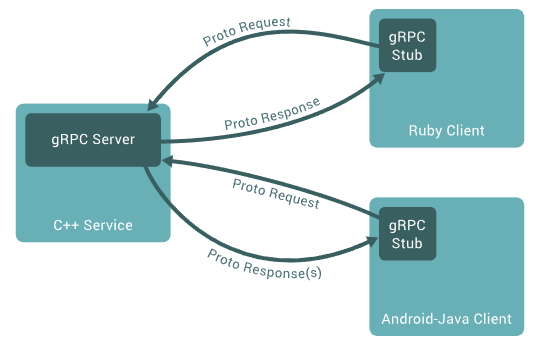
\includegraphics[width=\linewidth]{img/grpc-overview.png}
    \caption{Příklad komunikace serveru a různých klientů}
	\label{grpc-overview}
\end{figure}

\subsection{Principy a požadavky}
Níže jsem vybral několik hlavních principů a požadavků, na jejichž základě gRPC vzniklo. Všechny jsou pak dostupné na \cite{grpc_requirements}.
\begin{itemize}
    \item Služby a zprávy - Podpora filozofie mikroslužeb a snaha od oproštění se od problémů s distribuovanými objekty.
    \item Pokrytí a jednoduchost - gRPC by mělo být dostupné na všech populárních vývojových platformách a zároveň dostatečně jednoduché pro sestavení na vlastní platformě.
    \item Zdarma a otevřené - všechny základní funkcionality by měly být dostupné zdarma
    \item Interoperabilita a dosah - protokol musí být schopný přežít cestu internetem
    \item Obecné a výkonné - gRPC musí být vhodné pro velkou škálu způsobů užití a zároveň musí zůstat výkonné
    \item Vrstvené - klíčové vrstvy protokolu se musejí vyvíjet nezávisle na sobě. Nesmí se stát, že úprava na síťové vrstvě způsobí přeřuší chod na vrstvě aplikační.
    \item Blokujících a neblokujících operace - podpora synchronní a asynchronní komunikace mezi klientem a serverem je klíčová pro některé platformy.
    \item Standardizované stavové kódy - omezení množiny stavových kódů si klade za cíl jasnější očetřování chyb.
\end{itemize}

\subsection{Protocol buffer}
Můžeme mít například server implementovaný v Javě a pak několik klientských aplikací napsaných v různých jazycích, např. Javascriptu nebo Ruby, viz obrázek \ref{grpc-overview}. Aby mohla klientská aplikace volat vzdálené metody na serveru jako lokální, je potřeba zavést v jaké formátu si budou server a klient vyměňovat zprávy. K tomu se využívají \textit{Protocol buffers}, ikdyž je možné využívat i jiné formáty pokud je to potřeba. Je to opensourcový mechanizmus od Googlu jak serializovat strukturovaná data.

Prvním krokem který musíme udělat je definovat si strukturu zpráv v \textit{proto} souboru - jedná se o obyčejný textový soubor s  koncovkou proto. Základním stavebním prvkem jsou zprávy.To je nejmenší logický celek obsahující dvojice jméno a hodnota nazývané pole. Každá definice pole obsahuje typ, jméno a číslo pole. Soupis všech dostupných skalárních typů je k dispozici zde \cite{proto_scalars}

\begin{figure}[H]
\begin{minted}{protobuf}
    message Product {
        int64 id = 1;
        string name = 2;
        string description = 3;
        int64 price = 4;
        int64 quantity = 5;
        repeated ProductCategory categories = 6;
        ProductBrand brand = 7;
        ProductStatus status = 8;
    }
\end{minted}
\caption{Příklad protobuf zprávy}
\label{proto-message}   
\end{figure}

Každé pole má svoje unikátní číslo. Toto číslo identifikuje pole serializované v binárním formátu a nemělo by se měnit. Protože k zakódování čísel od 1 do 15 nám stačí jediný bajt, je vhodné tato čísla použít pro pole, která se ve zprávách budou vyskytovat velmi často. Může být dobrý nápad si některá čísla nechat volná pro budoucí potřebu.

Jedna věc, na kterou je potřeba si dát pozor při navrhování zpráv, je že pokud při parsování zprávy nějaký element chybí, jeho odpovídající pole bude naplněno výchozí hodnotou. Pro skalární pole po parsování nemůžeme určit zda se tato výchozí hodnota ve zprávě skutečně vyskytovala nebo nebyla vůbec nastavena. 

Jakmile máme definované zprávy, je potřeba použít kompilátor protocol buffer \mintinline{text}{protoc}, který pak vygeneruje přístupové třídy v našem zvoleném jazyce. Tyto třídy pak obsahují metody na získávání a nastavování dat do zpráv a také metody na serializaci a deserializaci.

\subsubsection*{Definice služeb}
gRPc je stejně jako většina RPC systémů založena na myšlence definování služeb, které pak definují své metody a jejich parametry. Je možné definovat čtyři typy služeb.

\begin{itemize}
    \item \textbf{Unary} - Klient pošle jeden požadavek na server a server mu pošle jednu odpověď zpět.
    \item \textbf{Server streaming} - Klient pošle jeden požadavek na server a odpovědí získá stream, ve kterém mu server zašle sekvenci zpráv. Klient čte data tak dlouho dokud mu chodí zprávy.
    \item \textbf{Client streaming} - Klient zasílá sekvenci zpráv na server. Jakmile klient dokončí posílání zpráv, počká až je server přečtě a vrátí mu odpověď.
    \item \textbf{Bidirectional streaming} - Klient a server posílají sekvenci zpráv pomocí read-write streamu. Tyto dva streamy operují nezávisle na sobě, takže klient a server mohou číst a posílat zprávy v jakémkoli pořadí.
\end{itemize}

Jako první věc, kterou musíme udělat, je specifikovat verzi protocol bufferu. Následně můžeme v proto souboru nadefinovat služby a metody, které budou dostupné klientům.

\begin{minted}{protobuf}
syntax = "proto3";

service ProductRegister {
    rpc GetProduct (GetProductRequest)
        returns (GetProductResponse) {};
}
\end{minted}
Metoda musí být vždy definována uvnitř nějaké služby - na příkladě  výše se jedná o službu \mintinline{text}{ProductRegister}. Poté už můžeme definovat samotnou metodu - první je klíčové slovo \mintinline{text}{rpc}, za kterým následuje jméno metody. A poté nadefinujeme vstupní a výstupní parametry této metody, které musí být typu zpráva.

\subsubsection*{Kompilace protocol bufferu}
Uvažujme zprávu \mintinline{protobuf}{Product} z příkladu \ref{proto-message} s polem  \mintinline{protobuf}{name} a cílový jazyk Javascript. Kompilátor pak vygeneruje třídu \mintinline{js}{Product} s metodou \mintinline{js}{setName(value)} a dalšími potřebnými metodami.

Protoc kompilátor poté ke kódu protocol buffer zpráv také vygeneruje gRPC klientský a serverový kód. Výstup kompilátoru pak záleží na naší zvolené platformě. Pro jazyk C++ vygeneruje odpovídající .h a .cc soubory s třídou pro každou zprávu definovanou v proto souboru. Pro Javu dojde k vygenerování odpovídajících .java tříd společně se speciální Builder třídou sloužící k výrobě instancí tříd jednotlivých zpráv.

Pokud však chceme používat gRPC s jazykem Javascript, máme na výběr dva způsoby. Prvním je načítat dynamicky deskriptory služeb a klientských stubů přímo ze samotných proto souborů pomocí knihovny \mintinline{text}{@grpc/proto-loader}.
Druhý způsob je použití kompilátoru. Dříve zmínený kompilátor protoc bohužel nepodporuje Javascript a je potřeba použít kompilátor \mintinline{text}{grpc_tools_node_protoc}, který je dostupný ve správci balíčků npm. Ten pak vygeneruje třídy zpráv a metody na jejich manipulaci.

\subsubsection*{Verzování}
Filozofie gRPC je taková, že služby by se měly snažit být co nejvíce zpětně kompatibilní. To má několik výhod - existující klienti budou nadále fungovat, stačí udržovat pouze jednu verzi služby a další. V gRPC jsou změny kategorizovány do tří kategorií.

\begin{itemize}
    \item \textbf{Non-breaking changes} - Patří sem například přidání nové služby, metody nebo pole do zprávy.
    \item \textbf{Binary breaking changes} - Tyto změny jsou non-breaking na úrovni protokolu gRPC, ale je potřeba aktualizovat klienty. Jedná se např. o odstranění pole nebo přejmenování zprávy.
    \item \textbf{Protocol breaking changes} - Patří sem například přejmenování pole, změna čísla pole nebo odstranění služby.
\end{itemize}

Protobuf podporuje verzování API specifikací verze do volitelného označení balíčku, např. \mintinline{protobuf}{package products.v1;}. 

\section{Node.js }
JavaScript byl vytvořen společností Netscape jako skriptovací nástroj pro manipulaci s webovými stránkami uvnitř prohlížeče. Tato společnost se také neúspšně snažila zavést prostředí \textit{Netscape LiveWire} pro běh JavaScriptu na serveru. Server-side JavaScript se tak stal populární až v roce 2009 s uvedením Node.js.

Node.js \cite{node} je open-sourcové a meziplatformní prostředí pro běh JavaScriptu. Je postavené na Google V8 JavaScript engine \cite{v8}, který je také jádrem prohlížeče Google Chrome.

Node.js aplikace běží v jediném procesu a pro příchozí požadavky nevytváří nová vlákna. Když node.js provádí I/O operaci, například. čtení ze sítě nebo databáze, místo blokování vlákna, Node.js bude pokračovat až po vrácení výsledku této operace. Toto umožňuje obsluhovat vysoký počet příchozích spojení bez potřeby správy vláken.

Jedna z největších výhod Node.js je, že umožňuje frontendovým vývojářům, kteří píšou klientský kód v JavaScriptu, psát serverový kód bez nuntnosti učit se další jazyk. 
Při psaní JavaScriptu pro Node.js nemáme dostupné žádné objekty jako document nebo window, které nam poskytuje prohlížeč. Máme ale kontrolu nad prostředím, můžeme si vybrat jakou verzi Node.js budeme používat a není potřeba řešit podporu pro všechny různé verze prohlížeče.

\subsection{npm}
npm \cite{npm}, plným jménem node package manager, je výchozí správce balíčků pro Node.js (alternativou je např. yarn\cite{yarn}). Sestává z klienta pro příkazovou řádku a online databáze balíčků, která se označuje jako npm registry.

\chapter{Návrh}
Aby srovnání co nejvíce odpovídalo realitě, vybral jsem si jako vzor pro API, které budu implementovat, eshop. Je to typický příklad, se kterým se vývojář může setkat při své práci a zároveň je tento vzor dost obecný na to, aby si čtenář mohl jednoduše převést na jiný. Pro popis api jsem zvolil specifikaci OpenAPI.

\subsection{OpenAPI}
OpenAPI 

\chapter{Použité technologie}

\chapter{Realizace}
\section{REST API}
\section{GraphQL API}
\section{gRPC API}

\chapter{Testování}

\chapter{Závěrečné srovnání}

\begin{conclusion}
	%sem napište závěr Vaší práce
\end{conclusion}

\bibliographystyle{csn690}
\bibliography{mybibliographyfile}

\appendix

\chapter{Seznam použitých zkratek}
% \printglossaries
\begin{description}
	\item[REST] Representational state transfer
	\item[RPC] Remote procedure call
	\item[XML] Extensible markup language
\end{description} 

\chapter{Obsah přiloženého CD}

%upravte podle skutecnosti

% \begin{figure}
% 	\dirtree{
% 		.1 readme.txt\DTcomment{stručný popis obsahu CD}.
% 		.1 exe\DTcomment{adresář se spustitelnou formou implementace}.
% 		.1 src.
% 		.2 impl\DTcomment{zdrojové kódy implementace}.
% 		.2 thesis\DTcomment{zdrojová forma práce ve formátu \LaTeX{}}.
% 		.1 text\DTcomment{text práce}.
% 		.2 thesis.pdf\DTcomment{text práce ve formátu PDF}.
% 		.2 thesis.ps\DTcomment{text práce ve formátu PS}.
% 	}
% \end{figure}

\end{document}
